% ---------------------------------------------------------------------------
% ---------------------------------------------------------------------------
% Modelo LaTex para preparação do documento final de Dissertação de Mestrado
% O modelo está em conformidade com ABNT NBR 14724:2011: 
% Programa de Pós-Graduação em Informática
% Universidade Federal de Alagoas
% Versão: v0.9
% ---------------------------------------------------------------------------
% ---------------------------------------------------------------------------

\PassOptionsToPackage{inline}{enumitem}

\documentclass[
	% -- opções da classe memoir --
	12pt,					% tamanho da fonte
	openright,				% capítulos começam em pág ímpar (insere página vazia caso preciso)
	twoside,					% para impressão em verso e anverso. Oposto a oneside
	a4paper,					% tamanho do papel. 
	% -- opções da classe abntex2 --
	chapter=TITLE,			% títulos de capítulos convertidos em letras maiúsculas
	%section=TITLE,			% títulos de seções convertidos em letras maiúsculas
	%subsection=TITLE,		% títulos de subseções convertidos em letras maiúsculas
	%subsubsection=TITLE,	% títulos de subsubseções convertidos em letras maiúsculas
	% -- opções do pacote babel --
	english,				% idioma adicional para hifenização
	%french,				% idioma adicional para hifenização
	%spanish,				% idioma adicional para hifenização
	brazil					% o último idioma é o principal do documento
]{abntex2}

% ---------------------
% Pacotes OBRIGATÓRIOS
% ---------------------
\usepackage[T1]{fontenc}			% Seleção de códigos de fonte.
\usepackage[utf8]{inputenc}		% Codificação do documento (conversão automática dos acentos)
\usepackage{lastpage}				% Usado pela Ficha catalográfica
\usepackage{indentfirst}				% Identa o primeiro parágrafo de cada seção.
\usepackage{color}						% Controle das cores
\usepackage{graphicx,graphicx}	% Inclusão de gráficos
\usepackage{epsfig,subfig}			% Inclusão de figuras
\usepackage{microtype} 				% Melhorias de justificação
% ---------------------
		
% ---------------------
% Pacotes ADICIONAIS
% ---------------------
\usepackage{lipsum}									% Geração de dummy text
\usepackage{amsmath,amssymb,mathrsfs}	% Comandos matemáticos avançados 
\usepackage{setspace}  								% Para permitir espaçamento simples, 1 1/2 e duplo
\usepackage{verbatim}								% Para poder usar o ambiente "comment"
\usepackage{tabularx} 								% Para poder ter tabelas com colunas de largura auto-ajustável
\usepackage{afterpage} 								% Para executar um comando depois do fim da página corrente
\usepackage{url} 										% Para formatar URLs (endereços da Web)
\usepackage{svg}
% ---------------------

% ---------------------
% Pacotes de CITAÇÕES
% ---------------------
\usepackage[brazilian,hyperpageref]{backref}	% Paginas com as citações na bibliografia
\usepackage[alf]{abntex2cite}				% Citações padrão ABNT (alfa)
%\usepackage[num]{abntex2cite}				% Citações padrão ABNT (numéricas)
% ---------------------

% Definição de diretório de imagens
\graphicspath{{imagens/}}

% Configurações de CITAÇÕES para abntex2
% --- 
% CONFIGURAÇÕES DE PACOTES
% --- 

% ---
% Configurações do pacote backref
% Usado sem a opção hyperpageref de backref
\renewcommand{\backrefpagesname}{Citado na~(s) página~(s):~}
% Texto padrão antes do número das páginas
\renewcommand{\backref}{}
% Define os textos da citação
\renewcommand*{\backrefalt}[4]{
	\ifcase #1 %
		Nenhuma citação no texto.%
	\or
		Citado na página #2.%
	\else
		Citado #1 vezes nas páginas #2.%
	\fi}%
% ---

% Inclusão de dados para CAPA e FOLHA DE ROSTO (título, autor, orientador, etc.)
% ---
% Informações de dados para CAPA e FOLHA DE ROSTO
% ---
\titulo{FRAMEWORK COMPUTACIONAL PARA ANÁLISE DE FADIGA EM DUTOS SUBMARINOS EM VÃO-LIVRE}
\autor{Weverton Marques da Silva}
\local{Maceió-AL}
\data{Dezembro de 2020}
\orientador{Adeildo Soares Ramos Júnior}
\coorientador{Eduardo Setton S. da Silveira}
\instituicao{%
  Universidade Federal de Alagoas --- UFAL
  \par
  Centro de Tecnologia
  \par
  Programa de Pós-Graduação em Engenharia Civil
}
\tipotrabalho{Dissertação (Mestrado)}
% O preambulo deve conter o tipo do trabalho, o objetivo,
% o nome da instituição e a área de concentração
\preambulo{Dissertação apresentada como requisito parcial para obtenção do grau de Mestre pelo Programa de Pós-Graduação em Engenharia Civil do Centro de Tecnologia da Universidade Federal de Alagoas.}
% ---


% Inclui Configurações de aparência do PDF Final
%  Configurações de aparência do PDF final
% NÃO ALTERAR!!!

% alterando o aspecto da cor azul
\definecolor{blue}{RGB}{41,5,195}

% informações do PDF
\makeatletter
\hypersetup{
     	%pagebackref=true,
		pdftitle={\@title}, 
		pdfauthor={\@author},
    		pdfsubject={\imprimirpreambulo},
	    pdfcreator={LaTeX with abnTeX2},
		pdfkeywords={abnt}{latex}{abntex}{abntex2}{trabalho acadêmico}, 
		colorlinks=true,       		% false: boxed links; true: colored links
    		linkcolor=black,          	% color of internal links
    		citecolor=black,        		% color of links to bibliography
    		filecolor=black,      		% color of file links
		urlcolor=black,
		bookmarksdepth=4
} 
\makeatother
% --- 

% Inclui configurações da folha de rosto
\renewcommand{\folhaderostocontent}{
	\begin{center}
		\MakeUppercase{\imprimirautor}
		
		\vspace*{\fill}
		\vspace*{\fill}
		\textbf{\imprimirtitulo}
		
		\vspace*{\fill}
		\hspace{.45\textwidth}
		\begin{minipage}{.5\textwidth}
			\SingleSpacing
			\imprimirpreambulo
			
			\vspace*{1cm}
			\imprimirorientadorRotulo~\imprimirorientador
			\par
			\imprimircoorientadorRotulo~\imprimircoorientador
		\end{minipage}
		
		\vspace*{\fill}
		\vspace*{\fill}
		\imprimirlocal
		\par
		\imprimirdata
	\end{center}
}


% Configurações da fonte do texto
\usepackage{times}						% Usar a fonte Times New Roman
\renewcommand{\ABNTEXpartfontsize}{\normalsize}
\renewcommand{\ABNTEXsectionfontsize}{\normalsize}
\renewcommand{\ABNTEXsubsectionfontsize}{\normalsize}
\renewcommand{\ABNTEXsubsubsectionfontsize}{\normalsize}
\renewcommand{\ABNTEXsubsubsubsectionfontsize}{\normalsize}
\renewcommand{\ABNTEXchapterfontsize}{\normalsize}

%\chapterstyle{article}
\renewcommand{\ABNTEXchapterfont}{\fontseries{b}}

% O tamanho da identação do parágrafo é dado por:
\setlength{\parindent}{1.3cm}

% Controle do espaçamento entre um parágrafo e outro:
\setlength{\parskip}{0.2cm}  % tente também \onelineskip

% Espaço entre o título do capítulo e o texto
\setlength{\afterchapskip}{0.8cm}

% ---------------------
% Compila o índice
% ---------------------
\makeindex
% ---------------------

%%%%%%%%%%%%%%%%%%%%%%%%%%%
%%  INICIO DO DOCUMENTO  %%
%%%%%%%%%%%%%%%%%%%%%%%%%%%
\begin{document}

% Elementos textuais com numeração arábica
\pagenumbering{arabic}

% Retira espaço extra obsoleto entre as frases.
\frenchspacing

% ----------------------------------------------------------
% ELEMENTOS PRÉ-TEXTUAIS (Capa, Resumo, Abstract, etc.)
% ----------------------------------------------------------
\pretextual

% Capa
% ---
% Impressão da Capa
% ---
\begin{capa}
	\center
	UNIVERSIDADE FEDERAL DE ALAGOAS\\
	CENTRO DE TECNOLOGIA\\
	PROGRAMA DE PÓS GRADUAÇÃO EM ENGENHARIA CIVIL

	\vfill
	\MakeUppercase{\imprimirautor}

    \vfill
    \textbf{\imprimirtitulo}
    \vfill
    \vfill
    \imprimirlocal
    \par
    \imprimirdata

    \vspace*{1cm}
\end{capa}
% ---

% Folha de rosto (o * indica que haverá a ficha bibliográfica)
\imprimirfolhaderosto

% Imprimir Ficha Catalográfica
%% ---
% Ficha Catalográfica
% ---
% Isto é um exemplo de Ficha Catalográfica, ou ``Dados internacionais de
% catalogação-na-publicação''. Você pode utilizar este modelo como referência.
% Porém, provavelmente a biblioteca da sua universidade lhe fornecerá um PDF
% com a ficha catalográfica definitiva após a defesa do trabalho. Quando estiver
% com o documento, salve-o como PDF no diretório do seu projeto e substitua todo
% o conteúdo de implementação deste arquivo pelo comando abaixo:
%
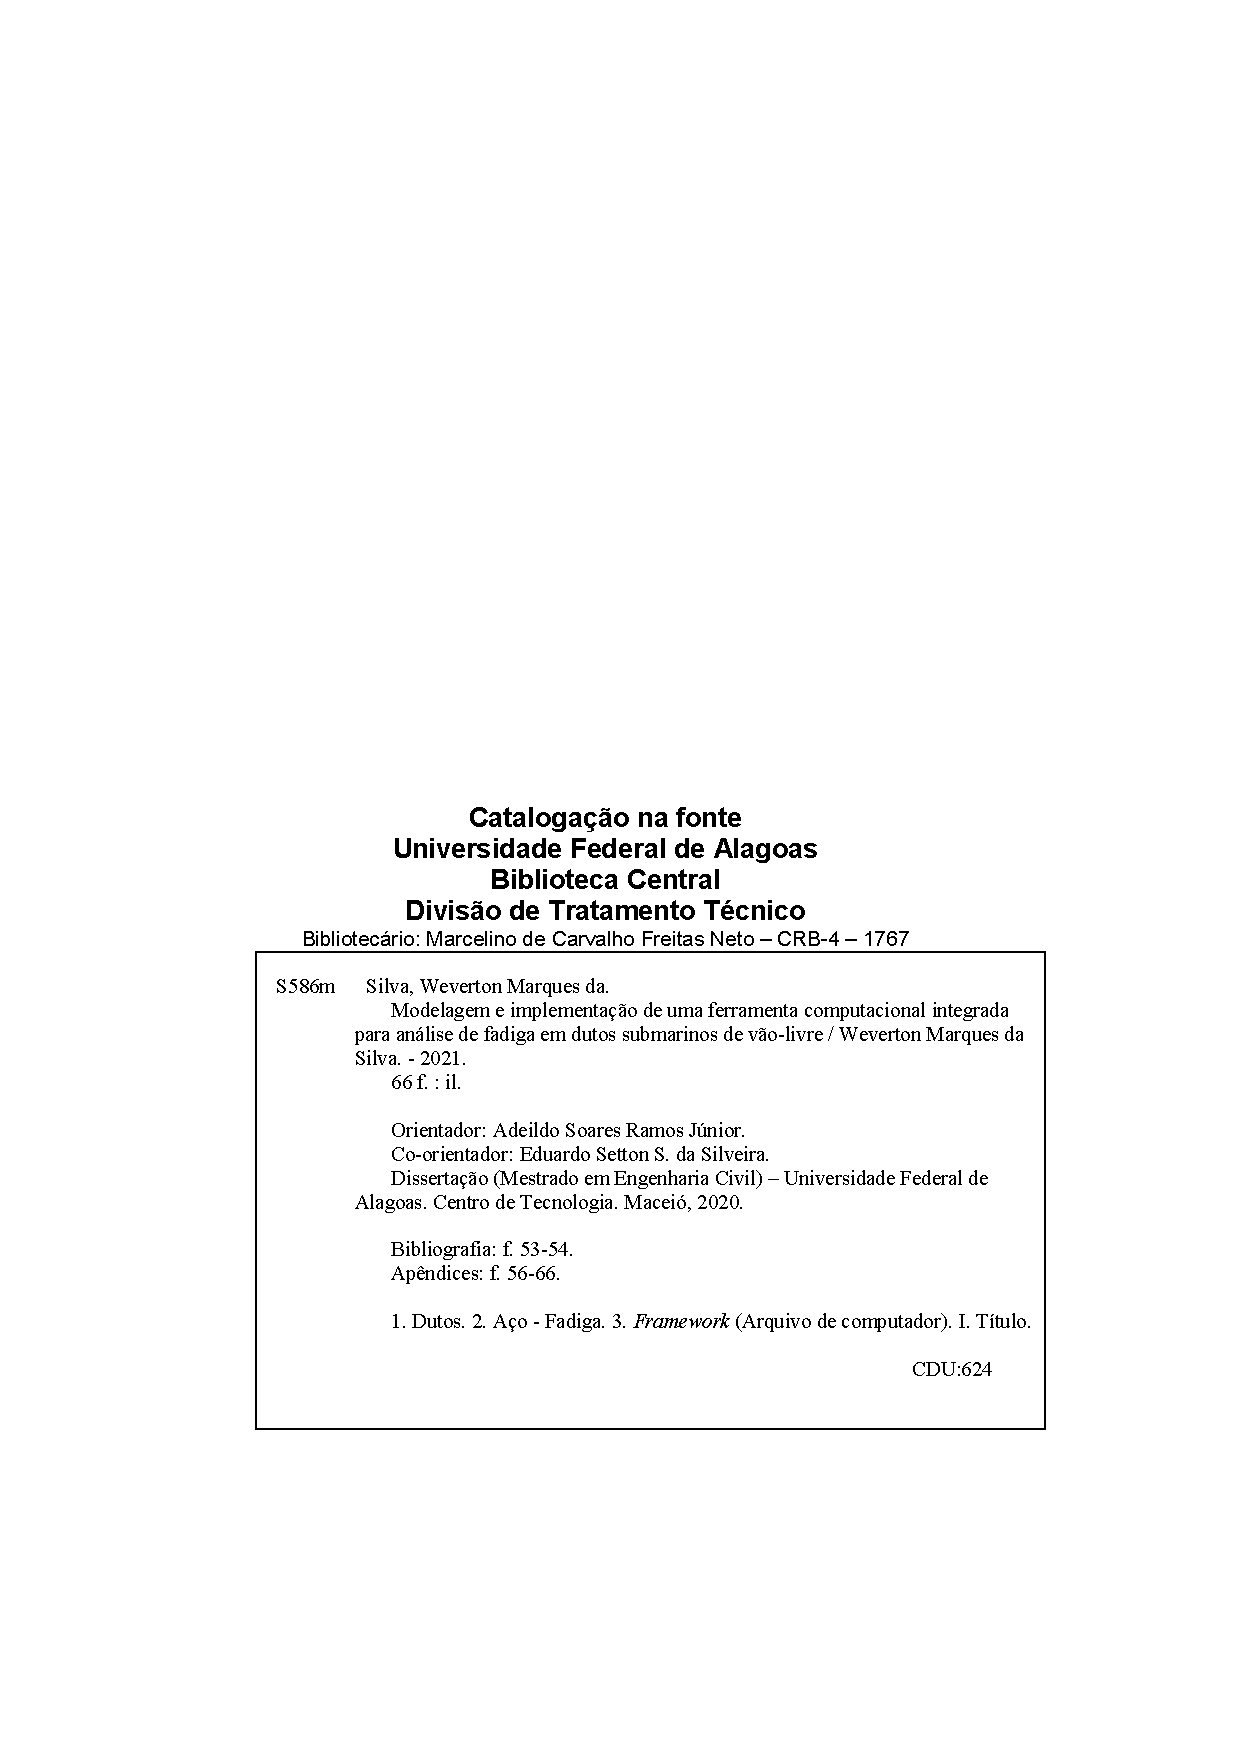
\includepdf{pretextual/ficha_catalografica.pdf}

% Inserir Folha de Aprovação
%% ---
% Assinaturas
% ---
% Isto é um exemplo de Folha de aprovação, elemento obrigatório da NBR
% 14724/2011 (seção 4.2.1.3). Você pode utilizar este modelo até a aprovação
% do trabalho. Após isso, substitua todo o conteúdo deste arquivo por uma
% imagem da página assinada pela banca com o comando abaixo:
%
% \includepdf{folhadeaprovacao_final.pdf}
%
\begin{folhadeaprovacao}
	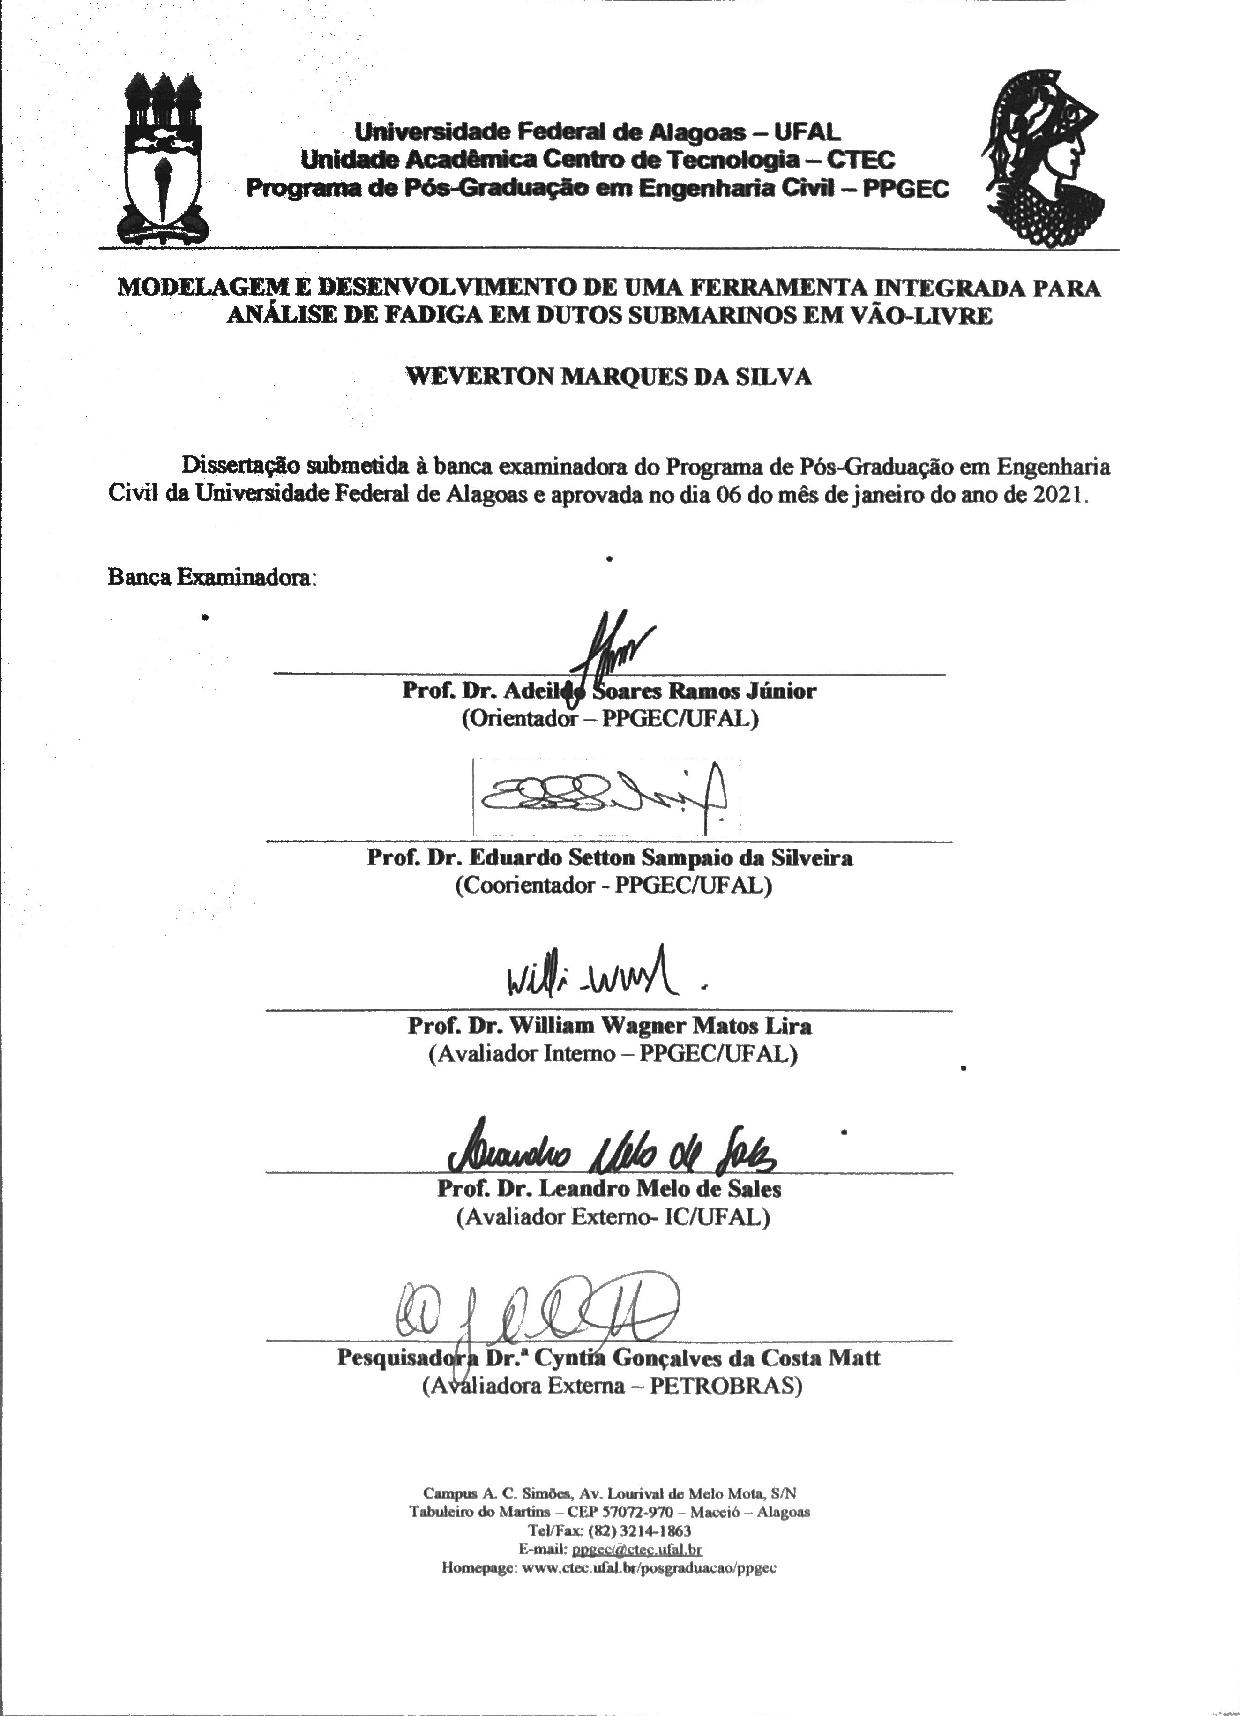
\includepdf{pretextual/folha_de_aprovacao}
	% \begin{center}
	% 	\textbf{Folha de Aprovação}
	% 	\vfill

	% 	AUTOR: \MakeUppercase{\imprimirautor}

	% 	\vfill
	% 	\imprimirtitulo
	% 	\vfill

	% 	\hspace{.45\textwidth}
	% 	\begin{minipage}{.5\textwidth}
	% 		\imprimirpreambulo
	% 	\end{minipage}%
	% 	\vfill

	% 	Trabalho aprovado. \imprimirlocal, 28 de setembro de 2016:
	% \end{center}

	% \assinatura{\textbf{\imprimirorientador} \\ Orientador}
	% \assinatura{\textbf{\imprimircoorientador} \\ Co-Orientador}
	% \assinatura{\textbf{William Wagner Matos Lira} \\ Convidado 1}
	% \assinatura{\textbf{Leandro Melo de Sales} \\ Convidado 2}

\end{folhadeaprovacao}

% Dedicatória
%% ---
% Dedicatória
% ---
\begin{dedicatoria}
   \vspace*{\fill}
   \centering
   \noindent
   \textit{ Aos meus pais XXXXXXXX e YYYYYYY, \\ por sempre estarem comigo em todos os momentos.} \vspace*{\fill}
\end{dedicatoria}
% ---

% Agradecimentos
%% ---
% Agradecimentos
% ---
\begin{agradecimentos}

Aos meus familiares por todo apoio. Especialmente, ao meus irmão, Wagner, e a minha noiva, Jhulia, que estiveram sempre ao meu lado e me ajudaram a encontrar a disposição para seguir em frente.

Agradeço ao meu orientador e coorientador pelos direcionamentos e por acreditaram na importância dos frutos desse trabalho.

Ao Laboratório de Computação Científica e Visualização pela minha participação no projeto IntegriSpan. Especialmente aos meus amigos Emerson, Josué, Jéssica e Renato. Sem a ajuda e parceria inestimável deles este trabalho não seria possível.

Aos professores do Programa de Pós-Graduação em Engenharia Civil que, com os conhecimentos transmitidos nas disciplinas, me ajudaram a elaborar esse trabalho.

\end{agradecimentos}
%% ---

% Epígrafe
%% ---
% Epígrafe
% ---
\begin{epigrafe}
    \vspace*{\fill}
	\begin{flushright}
		\textit{``Seja curioso. Leia muito. Experimente coisas novas.\\ Eu acho que muito do que as pessoas chamam de inteligência\\apenas se resume a curiosidade.''\\ % chktex 38
		          (Aaron Swartz)}
	\end{flushright}
\end{epigrafe}
% ---

% Resumo e Abstract
% ---
% RESUMOS
% ---

% RESUMO em português
\setlength{\absparsep}{18pt} % ajusta o espaçamento dos parágrafos do resumo
\begin{resumo}
TODO.

 \textbf{Palavras-chaves}: TODO.
\end{resumo}

% ABSTRACT in english
\begin{resumo}[Abstract]
 \begin{otherlanguage*}{english}
   TODO.

   \vspace{\onelineskip}
 
   \noindent 
   \textbf{Keywords}: TODO.
 \end{otherlanguage*}
\end{resumo}

% Lista de ilustrações
\pdfbookmark[0]{\listfigurename}{lof}
\listoffigures*
\cleardoublepage

% Lista de tabelas
\pdfbookmark[0]{\listtablename}{lot}
\listoftables*
\cleardoublepage

% Lista de abreviaturas e siglas
%\begin{siglas}
%  \item[ABNT] Associação Brasileira de Normas Técnicas
%  \item[abnTeX] Absurdas Normas para TeX
%\end{siglas}

% Lista de símbolos
%\begin{simbolos}
%  \item[$ \Gamma $] Letra grega Gama
%  \item[$ \Lambda $] Lambda
%  \item[$ \zeta $] Letra grega minúscula zeta
%  \item[$ \in $] Pertence
%\end{simbolos}

% Inserir o SUMÁRIO
\pdfbookmark[0]{\contentsname}{toc}
\tableofcontents*
\cleardoublepage

% ----------------------------------------------------------
% ELEMENTOS TEXTUAIS (Capítulos)
% ----------------------------------------------------------
\textual

% Ajusta o header para conter apenas o número da página
\pagestyle{simple}

% ----------------------------------------------------------
% TEXTO DA DISSERTAÇÃO
% ----------------------------------------------------------
\chapter{Introdução}
\label{chap:introdução}

\section{Planejamento de experimentos}
\label{sec:Exemplo de imagem}

\begin{figure}[!hbt]
	\centering
	\caption{Símbolo da UFAL}
	\label{fig:1_possuem_celular}
	
\includegraphics[width=0.25\textwidth]{imagens/ufal}
\end{figure}


\subsection{Teste 1}

\subsubsection{Teste 2}

\ref{chap:introdução}

% ----------------------------------------------------------
% ELEMENTOS PÓS-TEXTUAIS (Referências, Glossário, Apêndices)
% ----------------------------------------------------------
\postextual

\bibliography{bibliografia}

\end{document}
